\section{More Detailed Case Study}

\subsection{An Example of a Complete Retrieval Process}
\label{appendix::complete-log}

In \Cref{fig:complete-log}, we present a complete example of our retrieval process. This essentially illustrates the detailed procedure of the earlier Case Study in \Cref{fig:case-study-2}.

\begin{figure}
    \centering
    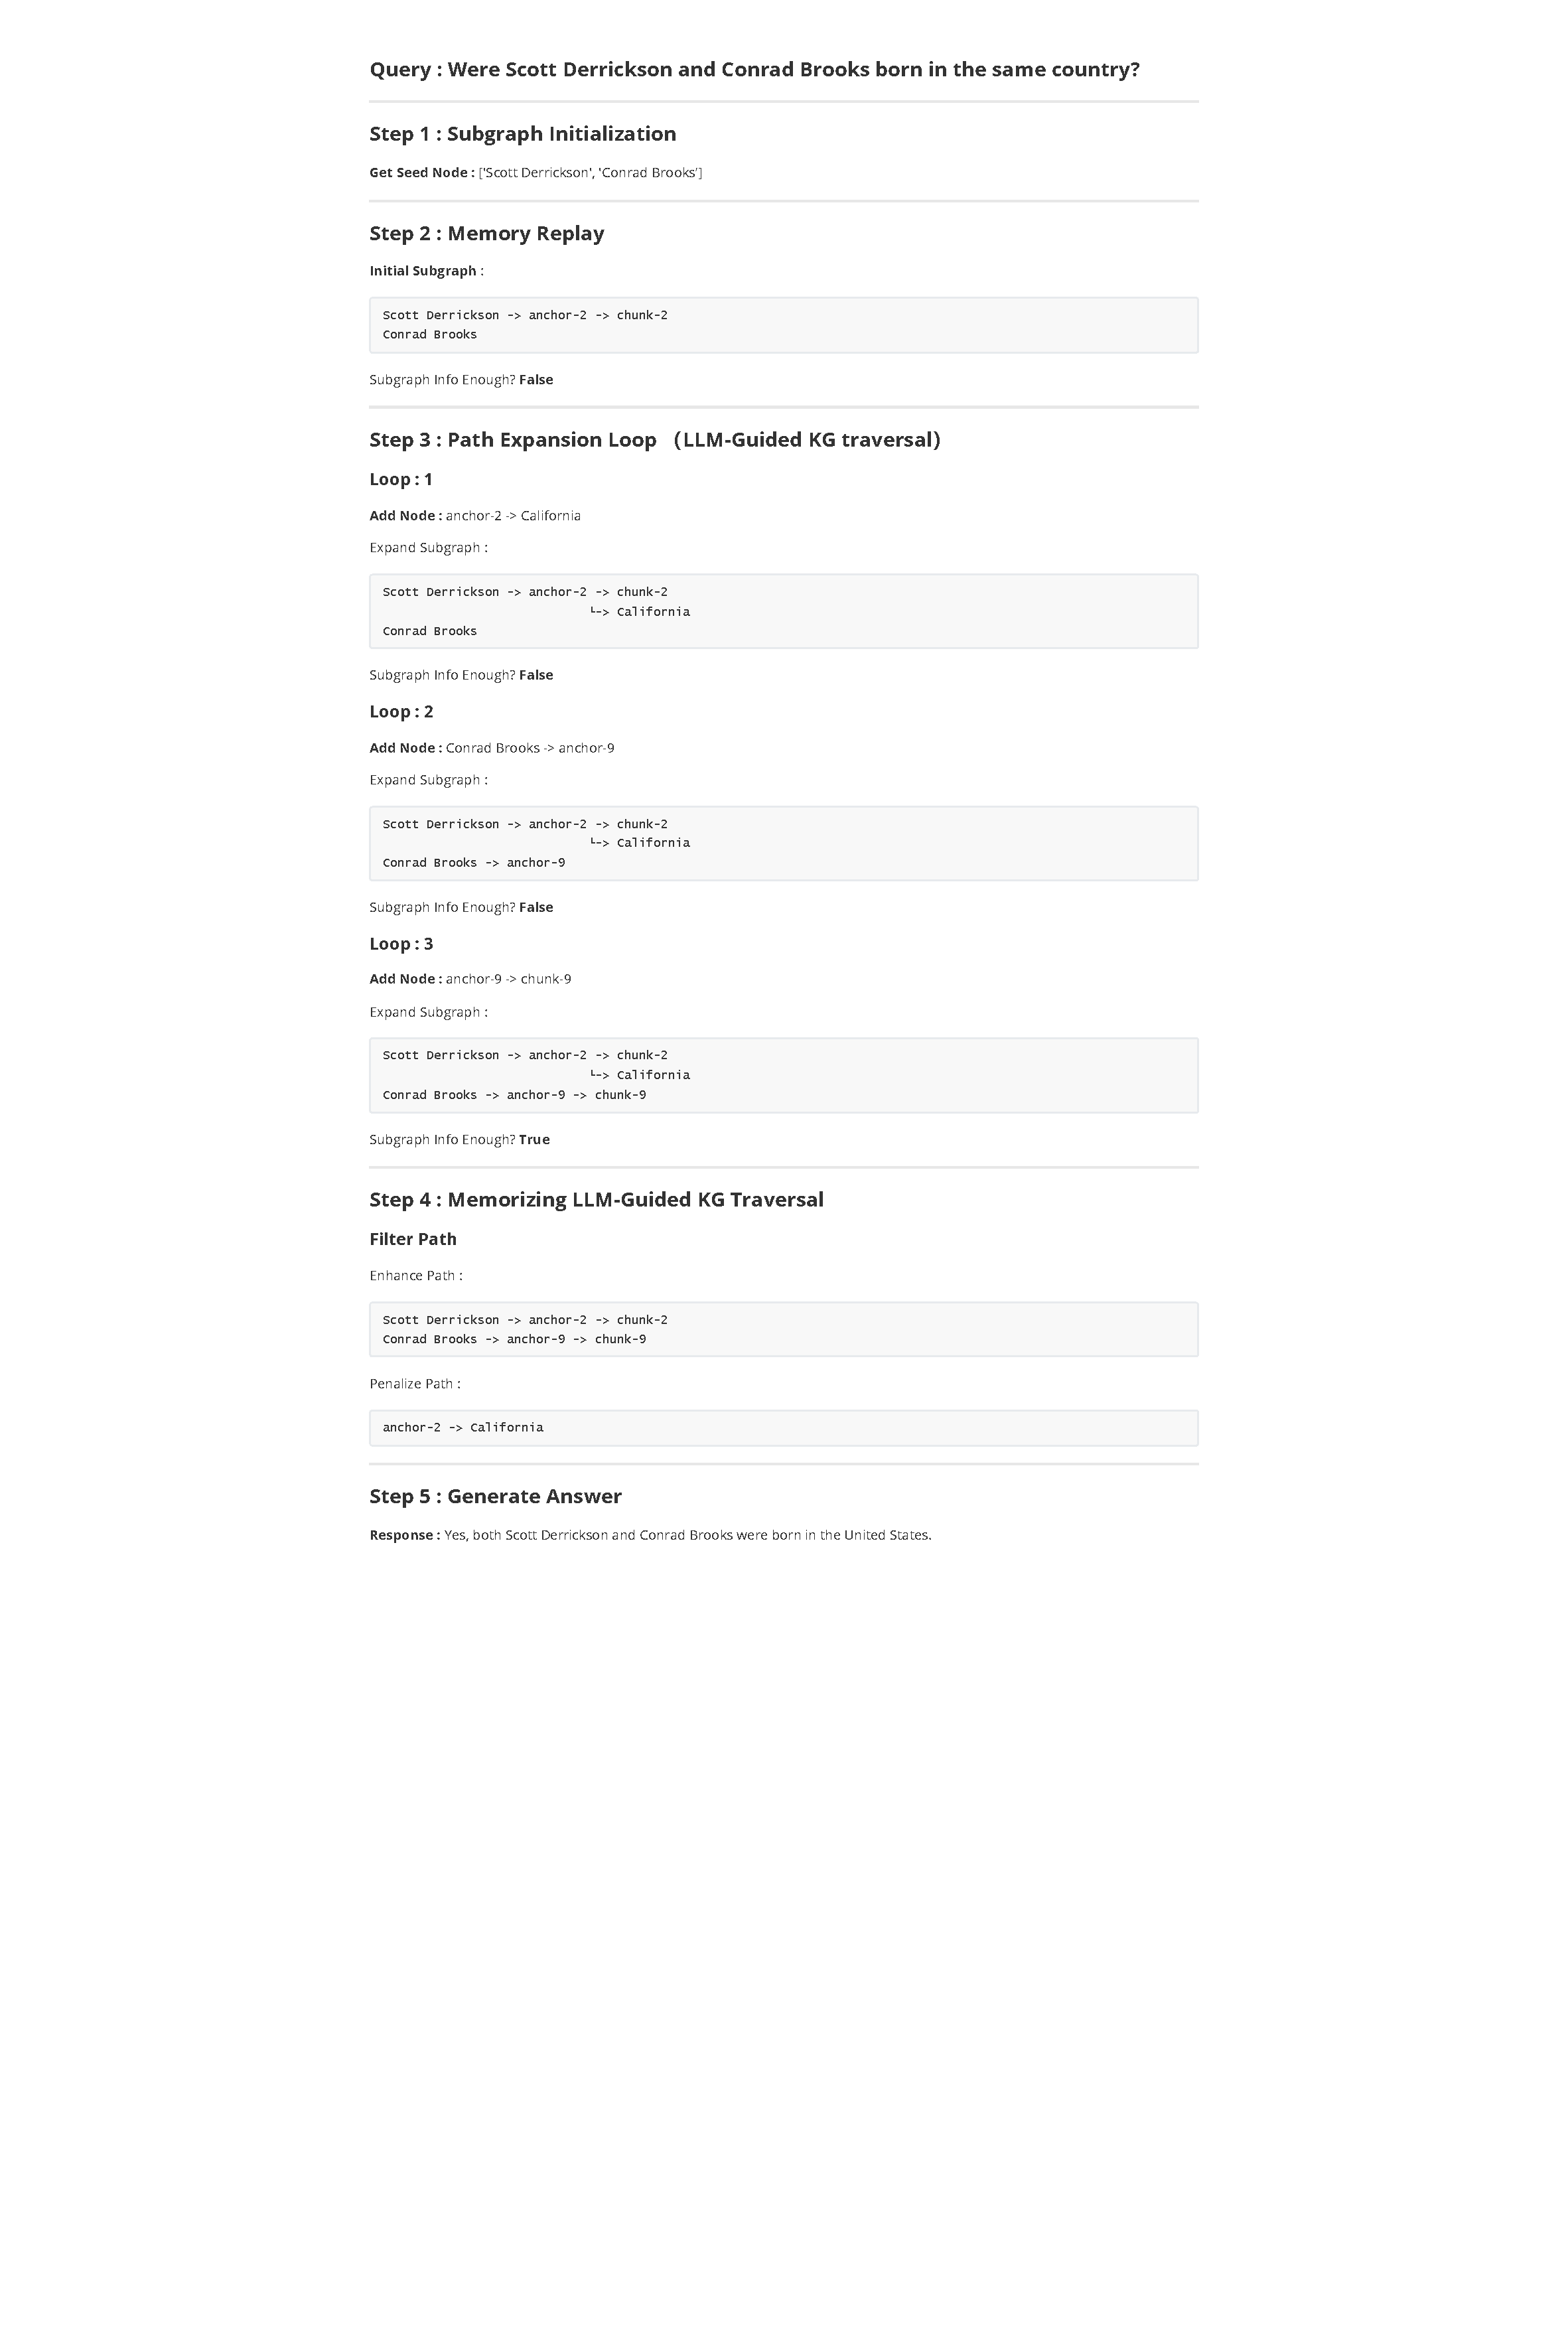
\includegraphics[width=\textwidth, height=\textheight, keepaspectratio]{Resources/log.pdf}
    \caption{An Example of a Complete Retrieval Process}
    \label{fig:complete-log}
\end{figure}

\subsection{WebUI Screenshots}
\label{appendix:webui-screenshots}

As shown in \Cref{fig:webui-case-study}, we present screenshots of \ours's web interface, which essentially correspond to the content of the earlier Case Study in \Cref{fig:case-study-1}.


\begin{figure}[htbp]
    \centering
    \begin{subfigure}[b]{0.45\textwidth}
        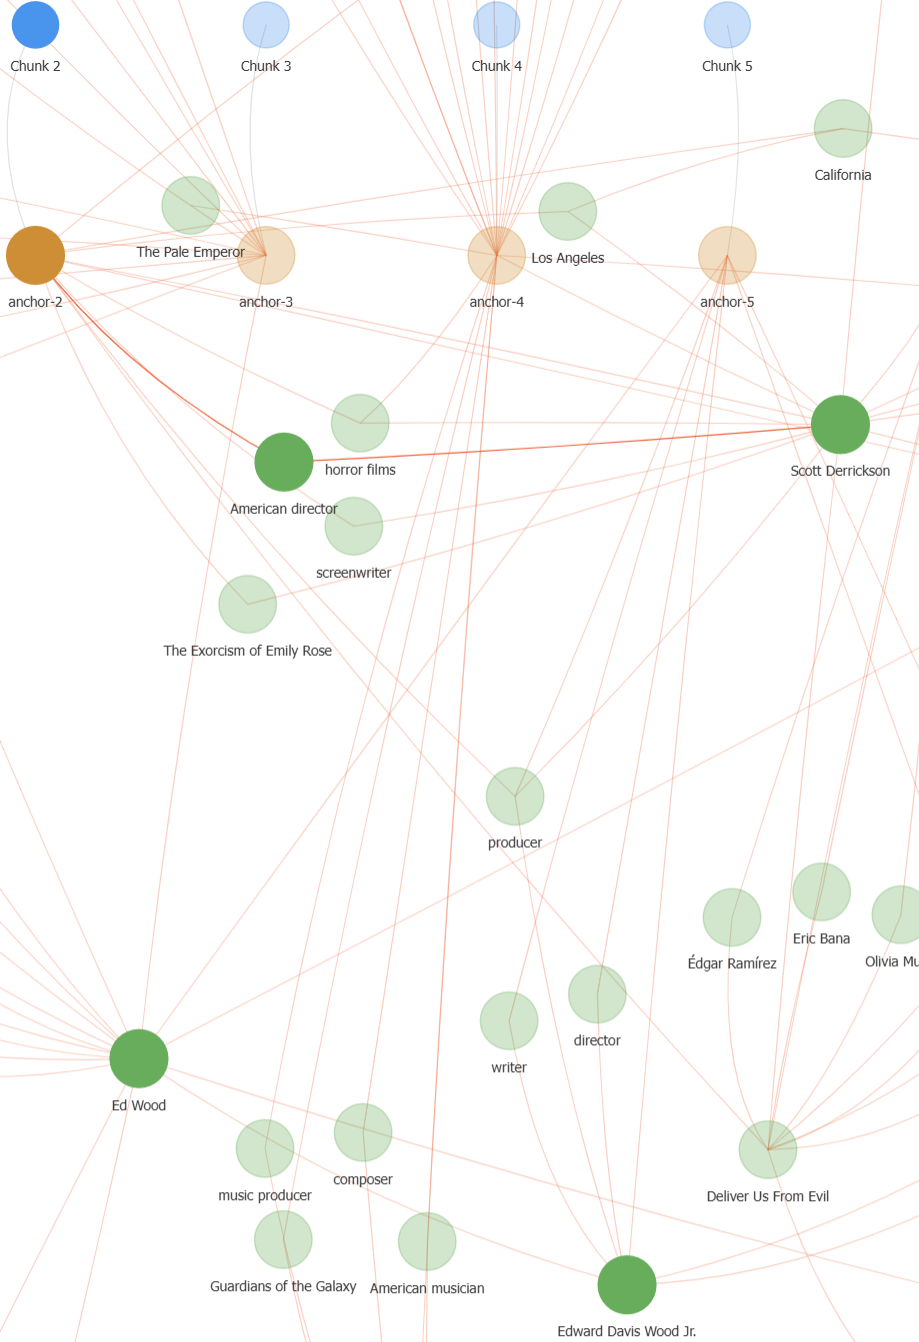
\includegraphics[width=\textwidth]{Resources/kg-update-before1.png}
        \caption{KG For First Query}
    \end{subfigure}
    \hfill
    \begin{subfigure}[b]{0.45\textwidth}
        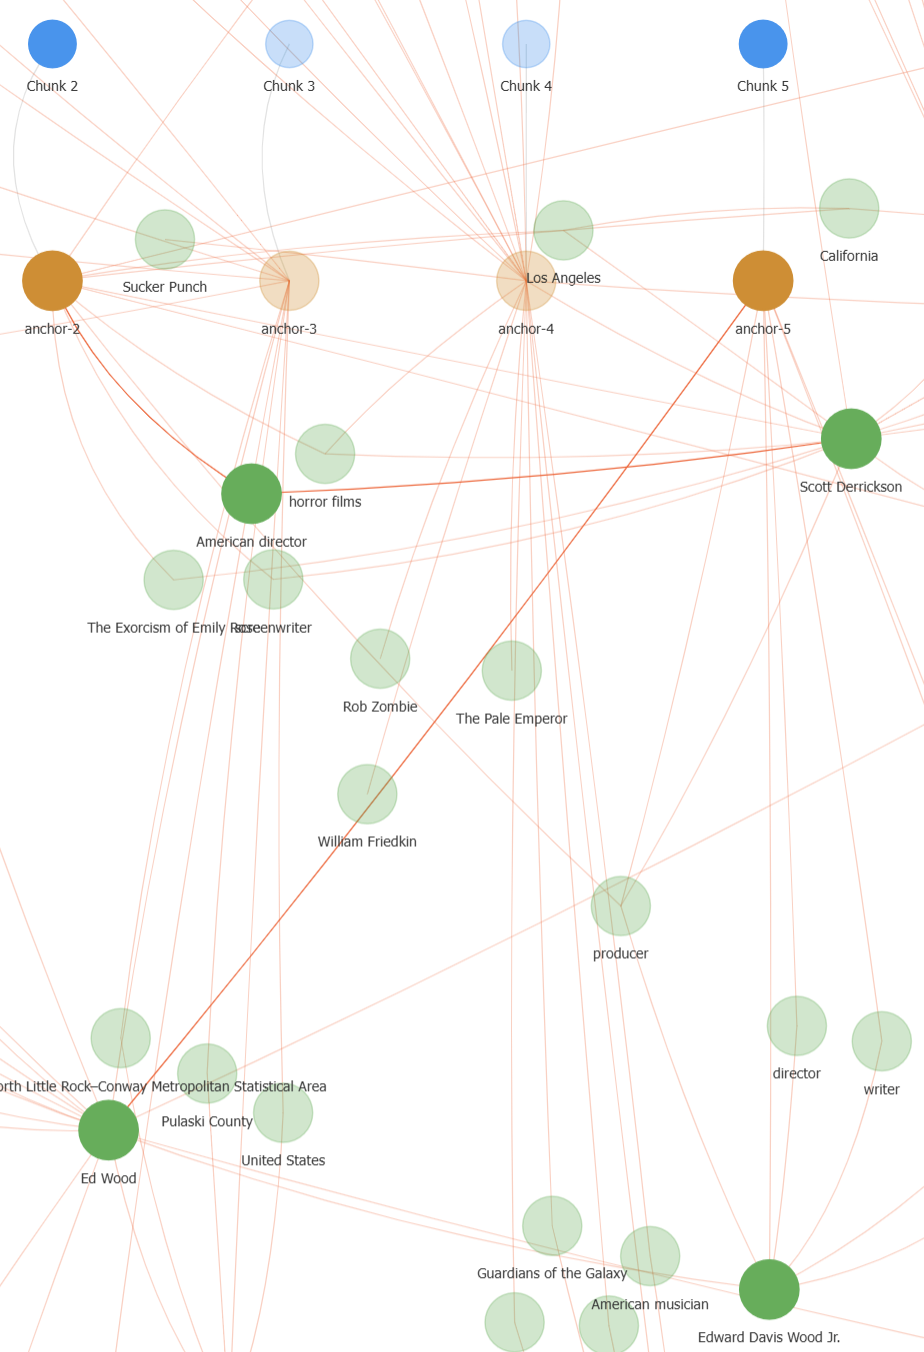
\includegraphics[width=\textwidth]{Resources/kg-update-after1.png}
        \caption{KG For Second Query}
    \end{subfigure}
    \caption{WebUI Screenshots}
    \label{fig:webui-case-study}
\end{figure}
